\documentclass[tikz, border=5mm]{standalone}
\usepackage{amsmath} % For text in math mode
\usetikzlibrary{arrows.meta} % For better arrowheads

\begin{document}
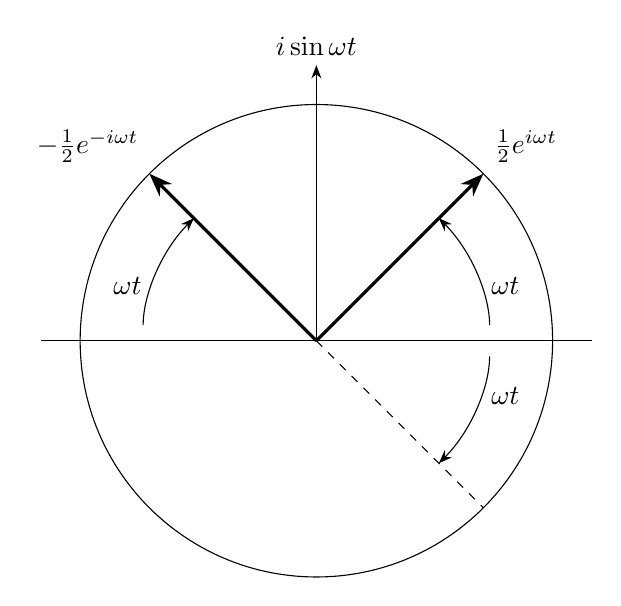
\begin{tikzpicture}
    % Define coordinates for the origin
    \coordinate (O) at (0,0);

    % Draw the circle
    \draw (O) circle (3cm);

    % Draw the axes
    \draw[-Stealth] (O) -- (0, 3.5cm) node[above] {$i \sin \omega t$};
    \draw (O) -- (3.5cm, 0);
    \draw (-3.5cm, 0) -- (O);

    % Draw the vectors
    \draw[-Stealth, very thick] (O) -- (2.121cm, 2.121cm) node[above right] {$\frac{1}{2}e^{i\omega t}$}; % For 45 degrees
    \draw[-Stealth, very thick] (O) -- (-2.121cm, 2.121cm) node[above left] {$-\frac{1}{2}e^{-i\omega t}$}; % For 135 degrees

    % Draw the angles
    % Angle for 1/2 e^(iwt)
    \draw[arrows={-Stealth}, shorten <=2mm] (2.2cm, 0) arc (0:45:2.2cm);
    \node at (2.4cm, 0.7cm) {$\omega t$};

    % Angle for -1/2 e^(-iwt)
    \draw[arrows={-Stealth}, shorten <=2mm] (-2.2cm, 0) arc (180:135:2.2cm);
    \node at (-2.4cm, 0.7cm) {$\omega t$};

    % Draw the dashed line for the negative angle
    \draw[dashed] (O) -- (2.121cm, -2.121cm); % For -45 degrees

    % Angle for the dashed line
    \draw[arrows={-Stealth}, shorten <=2mm] (2.2cm, 0) arc (0:-45:2.2cm);
    \node at (2.4cm, -0.7cm) {$\omega t$};

\end{tikzpicture}
\end{document}